\documentclass[11pt, oneside]{article}   	%standardeinstellung
\usepackage{amsmath}				%damit du formeln eingeben kannst
\usepackage[parfill]{parskip}    			% neuer absatz durch leere zeile
\usepackage{graphicx}				% bilder einfügen
\usepackage[onehalfspacing]{setspace}	%1,5 facher zeilenabstand
\usepackage{hyperref}				%damit man links erstellen kann
\usepackage{float}					%intelligentes anpassen von bildern, damit es keine lücken im text gibt
\graphicspath{ {figures/} }				%automatisches erstellen von "List of Figures"
\usepackage[font=small,labelfont=bf]{caption} %formatierung der bildunterschrift
 \usepackage{geometry}				%Seitenlayout
 \usepackage{tikz}
 \usetikzlibrary{shapes,arrows}

 \geometry{						%musst du nicht unbedingt selbst einstellen
 a4paper,
 total={210mm,297mm},
 left=15mm,
 right=15mm,
 top=25mm,
 bottom=20mm,
 }
\usepackage{ragged2e}
\usepackage{amssymb}
\usepackage{caption}
\usepackage{natbib}
\usepackage[utf8]{inputenc}
\usepackage{amsmath}
\usepackage{amsfonts}
\usepackage{amssymb}
\usepackage{wrapfig}
\usepackage{subcaption}
\usepackage{pdflscape}
\usepackage{filecontents,url}
\usepackage{soul}
\usepackage[space]{grffile}
\usepackage[UKenglish]{isodate}

\def\checkmark{\tikz\fill[scale=0.4](0,.35) -- (.25,0) -- (1,.7) -- (.25,.15) -- cycle;}

\title{Progress Report for MPhil Thesis}
\author{Tilman Graff -- University of Oxford}
\date{\today}

\begin{document}

\tikzstyle{data} = [draw, ellipse, fill=blue!20,
    text width=4.5em, text centered, node distance=3cm, minimum height=4em]
\tikzstyle{input} = [draw, ellipse, fill=red!20,
    text width=4.5em, text centered, node distance=3cm, minimum height=4em]
\tikzstyle{output} = [draw, ellipse, fill=green!20,
    text width=4.5em, text centered, node distance=3cm, minimum height=4em]
\tikzstyle{program} = [rectangle, draw, fill=white!20,
    text width=5em, text centered, rounded corners, minimum height=4em]
\tikzstyle{line} = [draw, -latex']

\bibliographystyle{cantoni_copy}
\maketitle

\section*{Open Questions -- What I need to discuss}
Topics to be raised in my next supervisor meeting.

Below starts my latest progress report.

\noindent\rule{\textwidth}{0.4pt}

\section{Research Question}
\textbf{Which factors influence the global distribution of trade network optimality?}

In this thesis, I aim to create a (potentially) global -- in any case African -- dataset of trade network efficiency. Taking the spatial distribution of current economic activity and population as given, I use a model from a recent working paper to determine the optimal trade network for each country. I then compare each country's current road network to its optimal one and derive a measure of how far a country is currently away from its ideal self.

In a second step, I will then investigate the origins of this global distribution. Which factors led to the heterogeneities among countries today? Specifically, I will look at:

\begin{itemize}
  \item Do networks with large colonial infrastructure investments do better or worse today?
  \item Does tribal favoritism explain why some areas are lacking lucrative investment?
  \item And many more. See below.
\end{itemize}

Ferdinand notes that the better these questions are, the more I will be scrutinised for the methodology. But that's what I want!

\section{Research steps}

In order to conduct this research, I will need to follow a series of steps and transfer data between multiple programming softwares. Here is a step-by-step guide, with progress as of \today:



\begin{itemize}
  \item[\checkmark] Find global raster data on population, night-lights, ruggedness, and colonial infrastructure investments.
  \item[\checkmark] Grid the world on 50x50km squares and aggregate finer-resolution data into those grids.
  \item \st{Locate the maximum population point within each grid and call this the (population) centroid of the grid.} I decided against this additional step. Mostly because I cannot figure out how to do it in QGIS. (And it's probably not that important?). Instead, I investigate travel times and distances between unweighted geometric centroids.
  \item[\checkmark] Use OpenStreetMap to find distance and average speed between neighboring gridcells.
  \item[\checkmark] Use distance and ruggedness to calculate Infrastructure Building Cost Matrix $\delta^{I}_{i,k}$ for every country.
  \item[\checkmark]Use average speed to calculate current Infrastructure Matrix $I_{i,k}$ for every country.
  \item[\checkmark] Use distance to calculate (iceberg) Trade Constant Matrix $\delta^{\tau}_{i,k}$ for every country.
  \item Use $\delta^{I}_{i,k}$, $\delta^{\tau}_{i,k}$, and $I_{i,k}$ to find the optimal trade network $I^{*}_{i,k}$ and optimal tradeflows $Q^{*}_{i,k}$ for every country. This directly follows the \cite{fajgelbaum_optimal_2017} Working Paper. I know how to do this, I am however afraid that this might take too long.
  \item Compare $I_{i,k}$ and $I^{*}_{i,k}$ for every country to obtain a measure of network optimality $\zeta_{c}$ for every country $c$.
  \item Investigate heterogeneity in $\zeta_{c}$

\end{itemize}

The following flowchart visualises the process. It shows the path input data (red circles) take through various programming languages (white rectangles) and intermediate datasets (blue circles) into eventual findings (green circle).



\section{Notes on individual steps}

In this section, I provide a more detailed account of what I did in each of the above-mentioned steps.

\resizebox{1\textwidth}{!}{
\begin{centering}
\begin{tikzpicture}[node distance = 3cm, auto]
  \node [input] (Lights) {Night Lights};
  \node [input, below of=Lights] (Rugg) {Ruggedness};
  \node [input, above of=Lights] (Population) {Population};
  \node [program, right of=Lights] (QGIS) {QGIS};
  \node [data, right of=QGIS] (Centroids) {Grid Centroids};
  \node [program, right of=Centroids] (R) {R};
  \node [input, below of=Centroids] (Roads) {Road Network};
  \node [data, right of=R] (Infrastructure) {Infrastr. Matrix};
  \node [data, above of=Infrastructure] (Trade) {Trade Cost};
  \node [data, below of=Infrastructure] (Building) {Building Cost};
  \node [program, right of=Infrastructure] (Matlab) {Matlab};
  \node [data, right of=Matlab] (Opt) {Optimal Network};
  \node [program, below of=Building] (Stata) {Stata};
  \node [input, right of=Stata, node distance=4.5cm] (misc) {Expl. variables};
  \node [output, left of=Stata, node distance=4.5cm] (Findings) {Findings};

  \path [line] (Lights) -- (QGIS);
  \path [line] (Population) -- (QGIS);
  \path [line] (Rugg) -- (QGIS);
  \path [line] (QGIS) -- (Centroids);
  \path [line] (Centroids) -- (R);
  \path [line] (Roads) -- (R);
  \path [line] (R) -- (Infrastructure);
  \path [line] (R) -- (Trade);
  \path [line] (R) -- (Building);
  \path [line] (Building) -- (Matlab);
  \path [line] (Infrastructure) -- (Matlab);
  \path [line] (Trade) -- (Matlab);
  \path [line] (Matlab) -- (Opt);
  \path [line] (Opt) -- (Stata);
  \path [line] (Roads) -- (Stata);
  \path [line] (misc) -- (Stata);
  \path [line] (Stata) -- (Findings);

\end{tikzpicture}
\end{centering}
}


\subsection{Find global raster data}
I use two datasources to create a global raster dataset of relevant variables:
\begin{itemize}
\item Data on night lights, ruggedness, land suitability, altitude, malaria index, and precipitation comes from \cite{henderson_global_2018}. These are available on 25km x 25km grids. Most of the data are for the year 2010. These data are different from most used in the recent literature, as they are not top-coded at 65 but rather able to gain much finer differentiations in highly-lit areas. I follow the authors in bottom-coding the data at 0.00034 instead of zero to counteract noise at the bottom. Importantly, there are a couple of regions with NaN values for the \citeauthor{henderson_global_2018} light data: most notably over a stretch of the Algerian Sahara and over  Lake Victoria. Once aware of these, I am not too worried about these areas. I drop them from my here on.
\item For census-level spatial population data, I use the Gridded Population of the World (GPW) database from the \cite{socioeconomic_data_and_applications_center_gridded_2016}. These are available on much finer resolution. This database is for the year 2015.
\item For later analysis, I will try to investigate heterogeneity on the ethnicity level. Which ethnic groups are significantly under/overinvested in and how does this correlate with political violence etc. Data for this comes from \cite{michalopoulos_long-run_2016}.
\end{itemize}

Using GIS, I aggregated these datasets to a 1-by-1 degree global grid (roughly 50km x 50km), following \cite{fajgelbaum_optimal_2017}. In doing so, I take spatial sums of population, and spatial averages of lights, ruggedness, malaria, and weather data.

\subsection{Construct Centroids}
For each of these gridcells, I calculate the geometric centroid. I do not weigh by population in constructing this centroid, as I have been unable to figure out how to do this. Ferdinand notes that this is not important.

I then crop all global centroids that are not over land. This leaves me with 59,059 gridcells. Doing this, I am aware that I will lose information: I cut gridcells that might be partially over land, as soon as their centroid is not over land. This approach will, however, create equidistant centroid locations, so I'm really just playing one disadvantage against the other.

I then attribute the centroids with the lights, population, and other data from the underlying gridcell. Thus, I act as if all people and all economic activity of a given cell were concentrated on the single centroid point. This is because \citeauthor{fajgelbaum_optimal_2017}'s model calculates trade between nodes, not areas. I find this to be a reasonable model simplification.

\subsection{Construct Global Road database}
I calculate the optimal route between any centroid and each of its eight surrounding neigbours. In doing so, I rely on the open source online project \textsc{Open Street Maps} (OSM), which is comparable to \textsc{Google Maps}, but allows for unlimited use of its API. I scrape OSM with an R-Package called \texttt{osrmRoute}. This package takes start and destination locations, sends them to OSM, and comes back with the optimal route, distance, and speed in virtually no time. I am amazed by how fast this is.

Two problems present itself:
\begin{enumerate}
  \item OSM's data supply is user generated and hence biased towards more prosperous areas. However, since I mostly care about big highways, I doubt there are all too glaring ommisions. Also, I care about relative inefficiencies within a country, not cross-section differences between countries.
  \item I tell OSM to find the optimal route for a car. However, in many remote areas, cars don't get you from A to B. \texttt{osrmRoute} then desparately tries to locate the user onto the nearest street (which could be far away!). I hence scrape the entire loc-by-loc route, and calculate the walking distance to the nearest street (and the walking distance from the end of the supplied route to the actual endpoint). I do so by taking direct paths and imply a walking speed of 4 km/h. I then calculate whether walking the entire distance from A to B is faster (not shorter, but faster!) than the route supplied by \texttt{osrmRoute}. If so, I replace the route with the walking route.
\end{enumerate}

\begin{figure}[h]
\centering
\caption{Road Networks for different countries as scraped off OSM}

\begin{subfigure}[c]{0.48\textwidth}
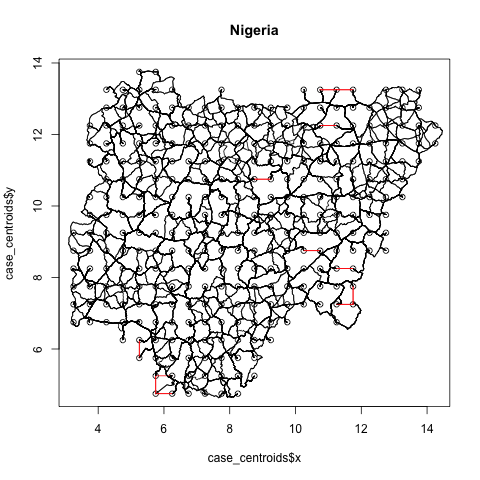
\includegraphics[width=\textwidth]{/Users/Tilmanski/Documents/UNI/MPhil/Second Year/Thesis_Git/Build/output/Road_Networks/network_Nigeria.png}
\caption{Nigeria}
\label{fig:nigeria}
\end{subfigure}
\begin{subfigure}[c]{0.48\textwidth}
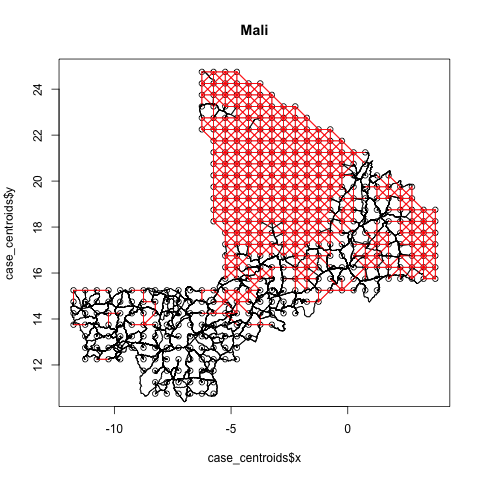
\includegraphics[width=\textwidth]{/Users/Tilmanski/Documents/UNI/MPhil/Second Year/Thesis_Git/Build/output/Road_Networks/network_Mali.png}
\caption{Mali}
\label{fig:Mali}
\end{subfigure}

\end{figure}

Figure \ref{fig:nigeria} displays how this would look like for the country of Nigeria. In black are optimal routes from all 289 centroids to their up to eight closest neighbours. If walking were the preferred option, this direct route is plotted in red. In Nigeria, this is mostly the case in some areas of the (swampy) South and East and some observations in the desert ridden North.

This procedure seems to well capture notions of remoteness: Consider the same graph but for Mali (Figure \ref{fig:Mali}). For much of the Saharan parts of the country, walking straight lines through the sand is the best available option. I am actually not too worried about these areas. They will presumably have almost no population or night lights and hence I do not expect the later optimisation to yield unrealistic trans-Saharan highways.

\section{Calibration of $I_{i,k}$, $\delta^{\tau}_{i,k}$, $\delta^{I}_{i,k}$}

Next up, I use the obtained matrices to construct underlying graph characteristics needed for the model to work. As rough guideline, I follow \cite{fajgelbaum_optimal_2017}.

\subsection{Current Infrastructure Network $I_{i,k}$}
The matrix $I_{i,k}$ discretises the road network obtained by \texttt{osrmRoute}. Basically, it attaches a value to each link between nodes, indicating ``How much infrastructure'' has been built into the edge. \cite{fajgelbaum_optimal_2017} do this by calculating the mean number of lanes a road has plus adding a dummy for national roads. I cannot do this, as I don't have comprehensive data on road lanes. However, I believe that the derived speed matrix from \texttt{osrmRoute} actually serves as the much more significant statistic for what \citeauthor{fajgelbaum_optimal_2017} want to capture. I hence propose
\begin{equation}
  I_{i,k} = \textrm{Average Speed}_{i,k}
\end{equation}

\begin{figure}[!b]
  \centering
  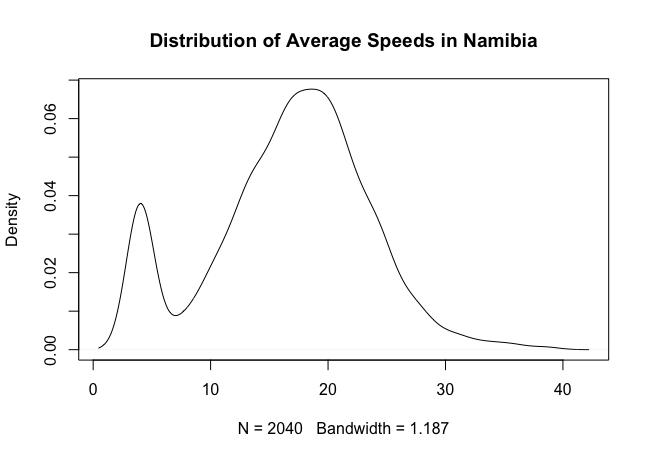
\includegraphics[width=0.7\textwidth]{/Users/Tilmanski/Documents/UNI/MPhil/Second Year/Thesis_Git/Build/output/Average Speeds/Speed_Namibia.png}
  \caption{Average Speed for Namibia, in km/h, 288 centroid locations}
  \label{fig:speed_namibia}
\end{figure}

This is obviously a very simple calibration. But the general logic is clear: if a certain edge allows a car to drive faster on it, chances are that more investments had been made into it. In a sense, this captures the same notion \citeauthor{fajgelbaum_optimal_2017} with their calibration based on lanes and national roads. Figure \ref{fig:speed_namibia} shows a distribution of the average speeds (on travelled routes, in km/h) for Namibia. As can be seen, the distribution follows a nicely behaved shape, with an additional hump at 4 km/h for purely walked routes (see above).

\begin{figure}[h]
\centering
\caption{Discretised Networks for different countries}

\begin{subfigure}[c]{0.48\textwidth}
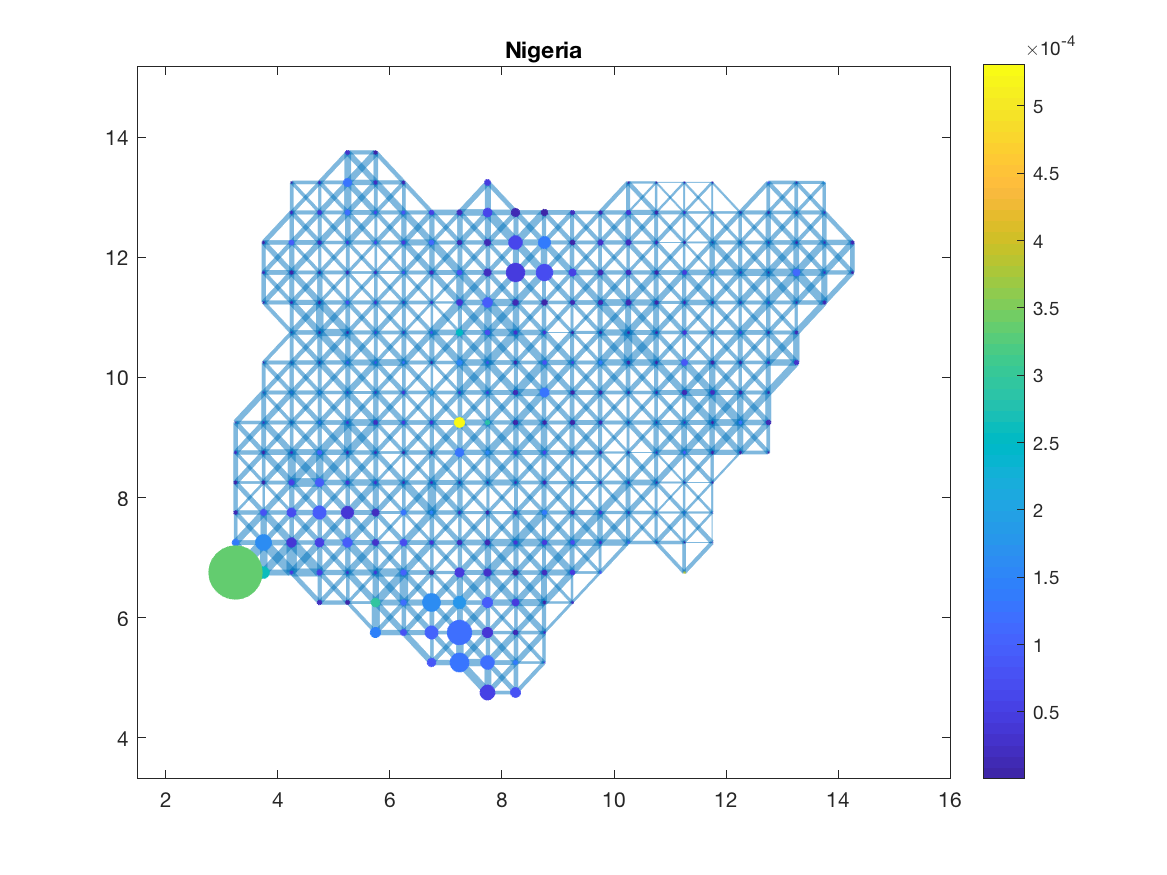
\includegraphics[width=\textwidth]{/Users/Tilmanski/Documents/UNI/MPhil/Second Year/Thesis_Git/Build/output/Matlab_graphs/initial_infrastructure/Nigeria_graph.png}
\caption{Nigeria}
\label{fig:nigeria_mat}
\end{subfigure}
\begin{subfigure}[c]{0.48\textwidth}
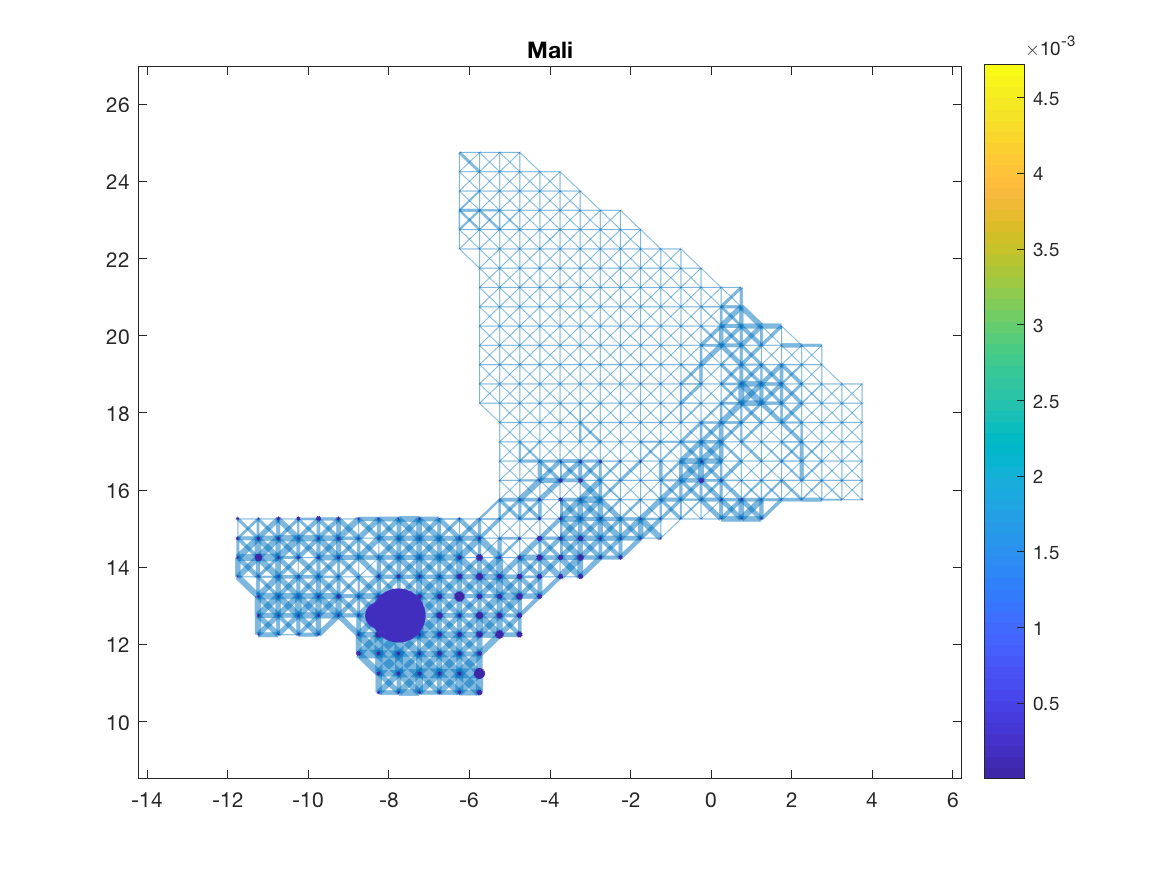
\includegraphics[width=\textwidth]{/Users/Tilmanski/Documents/UNI/MPhil/Second Year/Thesis_Git/Build/output/Matlab_graphs/initial_infrastructure/Mali_graph.png}
\caption{Mali}
\label{fig:Mali_mat}
\end{subfigure}

\end{figure}

With these calibrations, I can define country road networks as undirected graphs. Nodes correspond to centroid locations, edges correspond to their interconnections, with edgeweights defined by the average speed one reaches while driving (or walking) over the edge. Figure \ref{fig:nigeria_mat} and \ref{fig:Mali_mat} display this discretisation of the road network for Nigeria and Mali. Node sizes correspond to populations, node colours to implied productivity (see below), edge widths correspond to average speeds.

\subsection{Infrastructure Building Cost Matrix $\delta^{I}_{i,k}$}

I am still working on this one. The entries to this matrix represent the cost to building new infrastructure (think: one additional km/h to stay in the logic from above) onto a given edge from $i$ to $k$. \citeauthor{fajgelbaum_optimal_2017} use

\begin{equation}
  \textrm{ln}(\frac{\delta^{I}_{i,k}}{dist_{i,k}}) = \textrm{ln}(\delta_{0}^{I}) - 0.11*(dist_{i,k} > 50km) + 0.12*\textrm{ln}(\textrm{ruggedness}_{i,k})
\end{equation}

which comes from \cite{collier_cost_2015}. $\delta_{0}^{I}$ is individual for every country. I have all the data to replicate this,\footnote{Note that \citeauthor{henderson_global_2018} slightly alter the ruggedness variable, compared to \cite{nunn_ruggedness:_2012}, which also causes it to be on average a bit higher (about 20 per cent). Should not really matter.} but was thinking of including measures on extra low soil quality (which is congruent to Saharan soil) and (maybe) the Malaria index in there (or is that too much a colonial, \textit{``white guys walk in, build a road, and get Malaria''}, kind of thinking?). Update December 5th: I have now decided to just go with the \citeauthor{fajgelbaum_optimal_2017} calibration. \cite{collier_cost_2015} only have one additional variable in their dataset (which is population density), but that's not an underlying cost parameter and rather an outcome corollary. I will thus not include it and stick to \citeauthor{fajgelbaum_optimal_2017}.

\subsection{Iceberg Trade Constant Matrix $\delta^{\tau}_{i,k}$}

I cannot follow \citeauthor{fajgelbaum_optimal_2017} in this one, as their calibrations strike me as way to high. With their specification, I am basically stifling most trade as the cost is unbearable. To be fair, their parameters are calibrated on different measures for $I_{i,k}$ and $Y_{i}$, so it's not surprising that this does not work.

In trying to come up with a different approach, I find the analysis by \cite{atkin_whos_2015}, who estimate the trade cost elasticity to (log) distance as $0.0374$ for Ethiopia and $0.0558$ for Nigeria, using barcode-level spatial price data. I take the average value between the two and hence define

\begin{equation}
  \delta^{\tau}_{i,k} =  0.466*log(dist_{i, k})
\end{equation}

The actual iceberg trade costs are then computed as

\begin{equation}
  \tau_{i,k}(Q_{i,k}, I_{i,k}) = \delta^{\tau}_{j, k} * \frac{Q_{i,k}^{\beta}}{I_{i,k}^{\gamma}}
\end{equation}

where $Q_{i,k}$ represents trade flows between nodes (to capture notion of congestion), $I_{i,k}$ is the existing Infrastructure Network (derived above), $\beta = 1$ and $\gamma = 1$ in the easiest calibration.

With this, my estimates of $\tau_{i,k}(Q_{i,k}, I_{i,k})$ are much smaller than in \cite{fajgelbaum_optimal_2017}, but the resulting trade flows seem to be ok. I will have to do some fine tuning on this.

\subsection{Derive productivity measures}

I need a spatial distribution of innate productivity characteristics for each location. Since I have population and lights data, this should be relatively easy to back out. However, I initially confronted some problems with this. Firstly, I only have lights data and not GDP data. Is it fair to say that people produce lights and hence in a production function like

\begin{equation}
  Y_{i} = z_{i}L_{i}^{\alpha}
\end{equation}

lights can readily serve as $Y_{i}$? And if so, how can I circumvent the inevitable outlier-cell with hardly any population, but some remnant of lights, that will immediately render it hyperproductive? I used a couple of steps:

\begin{enumerate}
  \item All cells with no population are immediately coded as no productivity.
  \item I decide on $\alpha = 0.7$ to circumvent a problem of overvaluing the contribution of small populations.
  \item Then, $z_{i} = \frac{Y_{i}}{L_{i}^{\alpha}}$ and can be readily computed for the entire dataset.
\end{enumerate}

Results are promising. Capital cities tend to be more productive (even when they are bigger) than less populous cells. I should be able to go from here.

\subsection{Heterogeneous goods}
The original model allows for differentiated goods (which aggregated in canonical CES form). I think this is a very useful property. However, it also blows up computation time, as for every new good adds another price field over which to optimise. I tried various ways to have 5, 10, or even 20 different goods, but while they produce fancy graphs for small countries, they are just not computationally feasable in large countries.

I hence propose the following compromise:
\begin{enumerate}
  \item I introduce two different goods, an \emph{urban good} and an \emph{agricultural good}. Cities only produce the former, rural areas only produce the later (i.e. the respective productivity on the other good is zero.)
  \item To identify urban areas, I code the most densely populated gridcells as urban and the least densely populated as rural.
  \item I iteratively define the cutoff point for this as to match a country's 2016 total urbanisation rate, as reported by \cite{the_world_bank_world_2017}.\footnote{I start by assuming every location is a city and then gradually proceed to kick out the least densely populated locations, until the ratio of people living in urban areas to total population equals that of the WDI.} With this procedure, 7.3 per cent of locations are urban, but are home to 40 per cent of the population in the sample. A ratio which neatly compares to recent figures from \cite{lall_africas_2017}.
\end{enumerate}

\section{Computation of Optimal Networks}
After all this heavy data lifting and calibration, I can now finally start to actually get the Matlab Code up and running. Since it takes long for larger countries, I've started with the smaller ones. Over one night, the code can calculate the optimal reallocation of a given transport network for the 40 smallest African countries, or the three biggest. Below is how some of this looks for the country of Gabon.

\begin{figure}[!h]
\centering

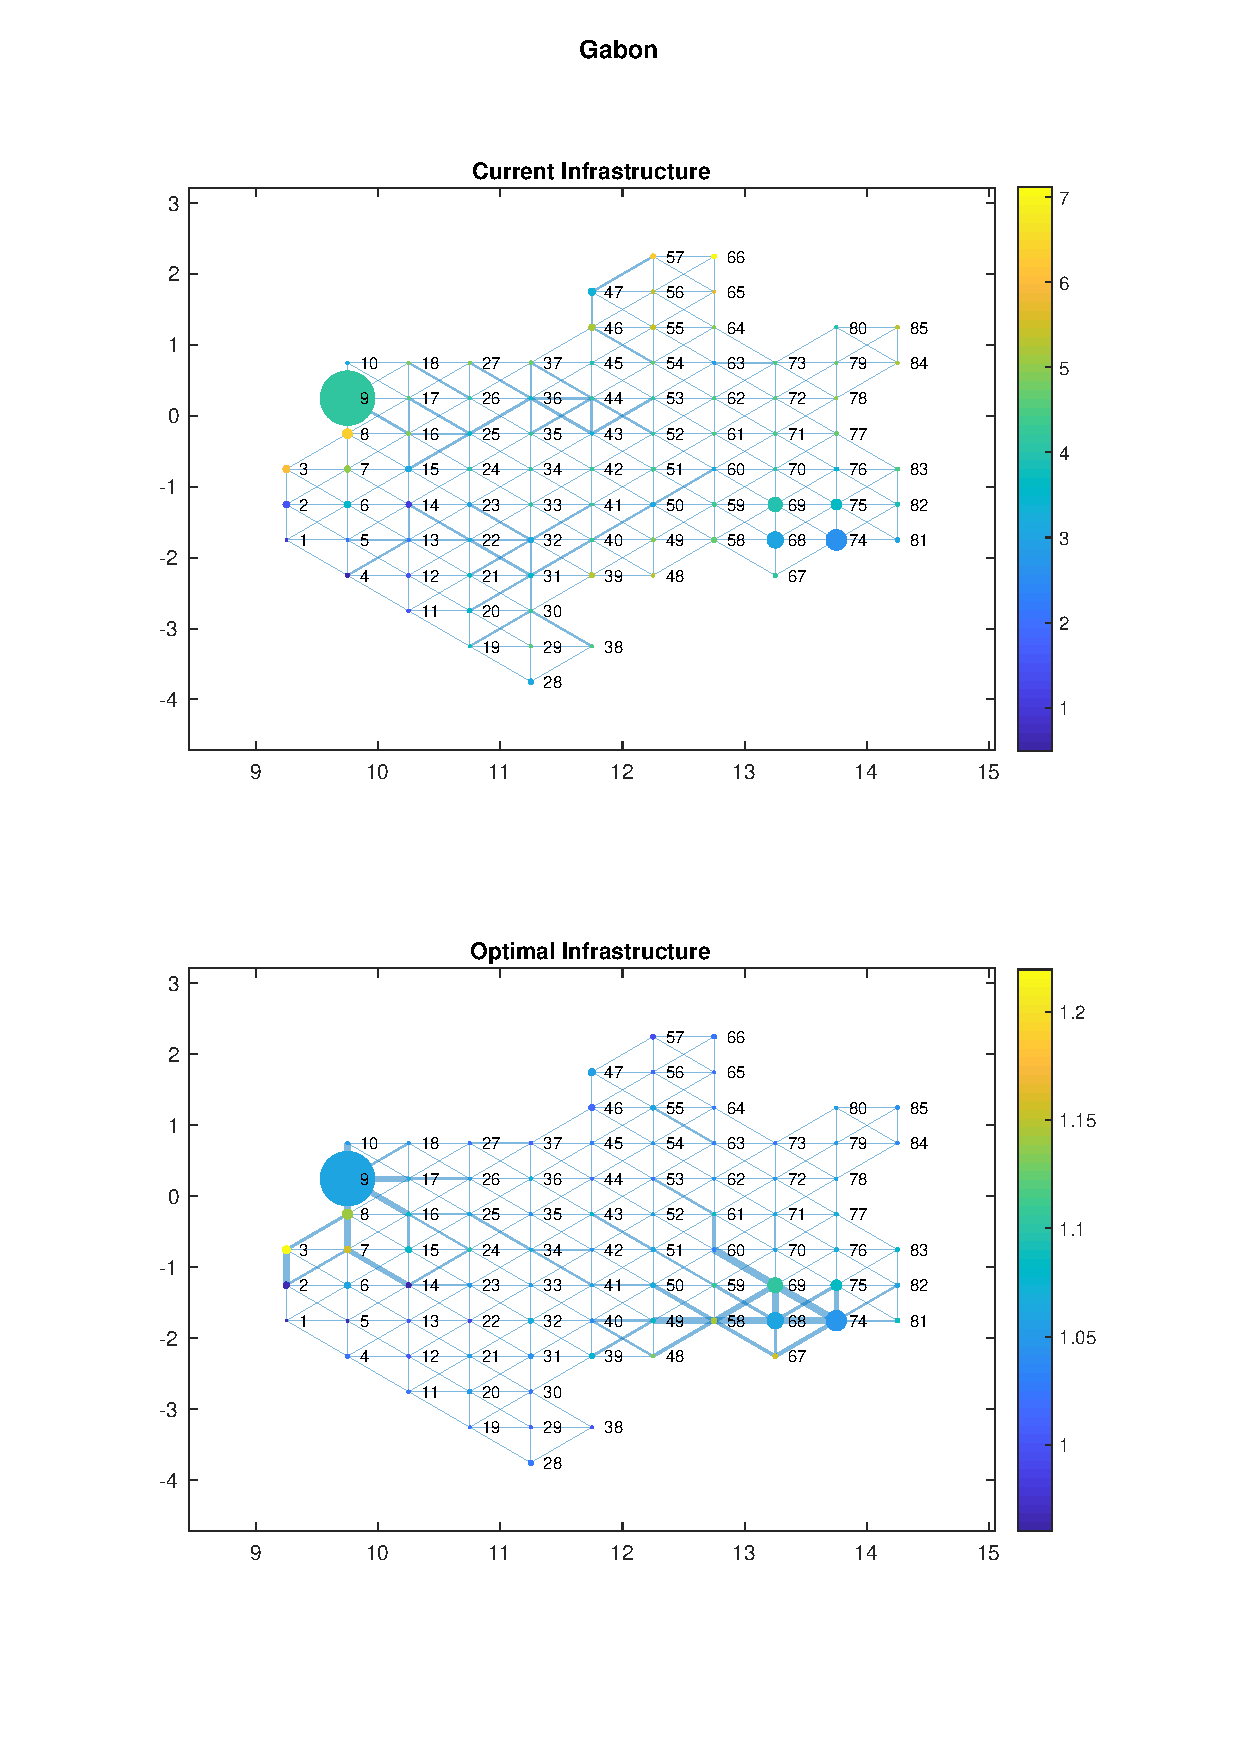
\includegraphics[width=0.9\textwidth]{/Users/Tilmanski/Documents/UNI/MPhil/Second Year/Thesis_Git/Build/output/Matlab_graphs/optimised_network/Gabon_graph.pdf}
\caption{Optimal reallocation for Gabon}
\label{fig:reall_gabon}

\end{figure}

From this, one can easily derive a measure of how much welfare a country or even region would gain under this optimal reallocation procedure. For starters, I just calculated welfare gains as

\begin{equation}
  \zeta_{c} = \frac{\textrm{Welfare under the optimal Infrastructure}_{c}}{\textrm{Welfare under the current Infrastructure}_{c}}
\end{equation}

Note that for entire countries, $\zeta_{c} \geq 0$ by construction. For individual regions, however, $\zeta_{c}$ can take on any positive value, really.

\begin{figure}[h]
\centering
\caption{Spatial Distribution of $\zeta_{c}$ for sample countries}

\begin{subfigure}[c]{0.3\textwidth}
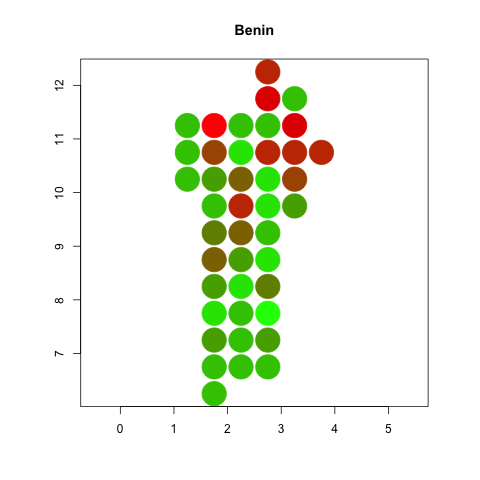
\includegraphics[width=\textwidth]{/Users/Tilmanski/Documents/UNI/MPhil/Second Year/Thesis_Git/Analysis/output/zeta_heatmaps/Benin_zeta.png}
\caption{Benin}
\label{fig:Benin_zeta}
\end{subfigure}
\begin{subfigure}[c]{0.3\textwidth}
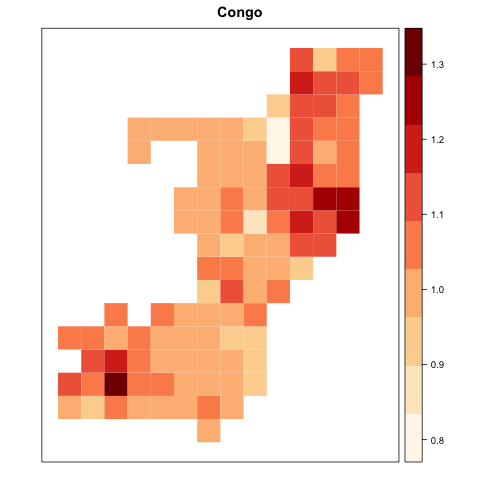
\includegraphics[width=\textwidth]{/Users/Tilmanski/Documents/UNI/MPhil/Second Year/Thesis_Git/Analysis/output/zeta_heatmaps/Congo_zeta.png}
\caption{Congo}
\label{fig:Congo_zeta}
\end{subfigure}
\begin{subfigure}[c]{0.3\textwidth}
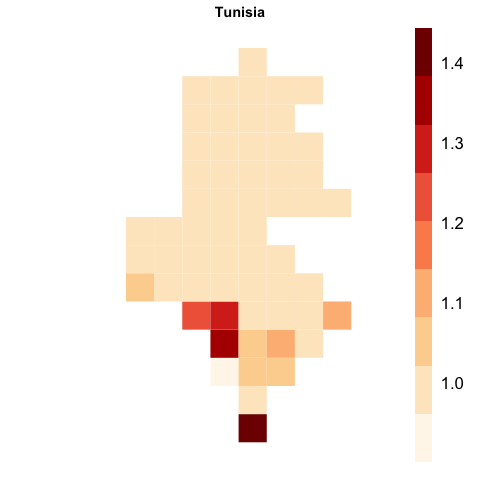
\includegraphics[width=\textwidth]{/Users/Tilmanski/Documents/UNI/MPhil/Second Year/Thesis_Git/Analysis/output/zeta_heatmaps/Tunisia_zeta.png}
\caption{Tunesia}
\label{fig:Tunisia_zeta}
\end{subfigure}

\end{figure}

Figures \ref{fig:Benin_zeta} to \ref{fig:Tunisia_zeta} show the spatial distribution of these welfare gains and losses under the optimal reallocation scenario.


\begin{table}[ht]
\centering
\caption{Sample Countries by $\zeta_{c}$}
\begin{tabular}{lr}
  \hline
Country & $\zeta_{c}$ in \% \\
  \hline
  South-Sudan & 6.66 \\
  Somalia & 4.76 \\
  Chad & 4.28 \\
  Gabon & 3.85 \\
  Democratic-Republic-of-the-Congo & 3.55 \\
  Madagascar & 3.16 \\
  Angola & 3.03 \\
  Guinea & 2.80 \\
  Ethiopia & 2.63 \\
  Sudan & 2.41 \\
  Niger & 2.25 \\
  Mozambique & 2.14 \\
  Uganda & 2.12 \\
  Liberia & 2.12 \\
  Mali & 2.06 \\
  Botswana & 2.03 \\
  Eritrea & 1.85 \\
  Central-African-Republic & 1.84 \\
  Namibia & 1.84 \\
  Zambia & 1.83 \\
  Cameroon & 1.76 \\
  United-Republic-of-Tanzania & 1.70 \\
  Kenya & 1.65 \\
  Burkina-Faso & 1.54 \\
  Sierra-Leone & 1.53 \\
  Burundi & 1.45 \\
  Zimbabwe & 1.36 \\
  Libya & 1.31 \\
  Rwanda & 1.27 \\
  Guinea-Bissau & 1.20 \\
  Mauritania & 1.09 \\
  Lesotho & 0.98 \\
  Benin & 0.95 \\
  Senegal & 0.90 \\
  Malawi & 0.87 \\
  Nigeria & 0.81 \\
  Togo & 0.77 \\
  Congo & 0.72 \\
  Cote-dIvoire & 0.72 \\
  Djibouti & 0.65 \\
  Equatorial-Guinea & 0.62 \\
  Ghana & 0.57 \\
  Western-Sahara & 0.57 \\
  South-Africa & 0.47 \\
  Morocco & 0.46 \\
  Algeria & 0.39 \\
  Egypt & 0.34 \\
  Tunisia & 0.24 \\
  Swaziland & 0.02 \\
   \hline
\end{tabular}
  \label{tab:national_zeta}
  \end{table}




I can also now rank all countries by the cumulative welfare gain they would achieve under the perfect reallocation scenario. Table \ref{tab:national_zeta} does so.

\section{Potential research alleyways}
$\zeta_{c}$ is representing whether an area would gain or lose with infrastructure under the optimal scenario. Broadly, there are two different pots of potential research questions. One has $\zeta_{c}$ on the LHS and one has it on the RHS:

\subsection{$\zeta_{c}$ on the LHS}
What determines why some areas are under-/overinvested in? Ideas could be
\begin{itemize}
  \item Colonial Legacies: do areas that had more colonial investment still enjoy more infrastructure than they should?
  \item Do areas from the ethnicity of the tribal leader enjoy too much infrastructure?
\end{itemize}

\subsection{$\zeta_{c}$ on the RHS}
This asks what the correlates / outcomes of being over/-underinvested in are. \cite{michalopoulos_long-run_2016} have a bunch of interesting outcomes like
\begin{itemize}
  \item Political Violence in frequency, intensity, and kind from ACLED
  \item Ethnic power relations from EPR dataset
  \item Wellbeing from DHS dataset
\end{itemize}

For these, the unit of observation would be ethnicities. So I would have to aggregate my $\zeta_{c}$ measure over the Murdock ethnicity map. Should be fine.

The trouble with both these approaches is that $\zeta_{c}$ is obviously both an outcome and an effect in the intricate interplay of the political economy of African countries. I don't know to what extend I can actually do inference, or will just have to rely on correlations. We'll see.


\section{Empirical results}
The following section merely records those regression results I find noteworthy.
\subsection{Grid-Level patterns}
My first set of investigations are being performed at the grid level. In general, OLS is run on a framework of the following sense
\begin{equation}
  \zeta_{i,c} = \alpha + \beta x_{i,c} + \delta_{c} + \sum_{a}^{}\gamma_{a} z_{i,c}^{a}
  \label{eq:regression}
\end{equation}
where $\zeta_{i,c}$ is the outcome of interest, the infrastructure gap of grid cell $i$ in country $c$. $x_{i,c}$ denotes the covariate of interest, $\delta_{c}$ is a country-fixed effect, and $z_{i,c}^{a}$ denote a set of potential controls. The coefficient of interest is $\beta$.

I have data on the exact positioning of all railroads built by colonial powers in every Sub-Saharan country. The data for every country but South Africa comes from \cite{jedwab_permanent_2016}. For South-Africa, I manually digitise an equivalent map printed in \cite{Herranz-Loncan_publicbenefitRailways_2017}. From these two sources, I also acquire information on railroads that were planned, but not built, giving a notion of ``Placebo Lines''. For each grid cell, I calculate the distance to the closest railroad (or placebo line) from the cell's centroid. I also calculate the total number of kilometres of colonial (actual and placebo) railroads in each gridcell.

\begin{table}[] \centering
  \caption{Colonial Railroads and Infrastructure Gap}
  \label{RailKM_zeta}
  \resizebox{0.9\textwidth}{!}{


  \begin{tabular}{@{\extracolsep{5pt}}lcccccc}
  \\[-1.8ex]\hline
  \hline \\[-1.8ex]
   & \multicolumn{6}{c}{\textit{Dependent variable: infrastructure gap $\zeta_{i}$}} \\
  \cline{2-7}
  \\[-1.8ex] & (1) & (2) & (3) & (4) & (5) & (6)\\
  \hline \\[-1.8ex]
   KM of colonial railroads & $-$0.0002$^{***}$ & $-$0.0001$^{***}$ & $-$0.0002$^{***}$ &  &  &  \\
    & (0.00004) & (0.00004) & (0.00004) &  &  &  \\
    & & & & & & \\
   KM of colonial placebo railroads &  &  &  & 0.00004 & $-$0.0002 & $-$0.0003 \\
    &  &  &  & (0.0003) & (0.0003) & (0.0003) \\
    & & & & & & \\
  \hline \\[-1.8ex]
  Country FE &  & Yes & Yes &  & Yes & Yes \\
  Geographic controls &  &  & Yes &  &  & Yes \\
  Observations & 10,158 & 10,158 & 10,158 & 10,158 & 10,158 & 10,158 \\
  R$^{2}$ & 0.001 & 0.099 & 0.111 & 0.00000 & 0.098 & 0.110 \\
  \hline
  \hline \\[-1.8ex]
  \textit{Note:}  & \multicolumn{6}{r}{$^{*}$p$<$0.1; $^{**}$p$<$0.05; $^{***}$p$<$0.01} \\
  \end{tabular}

}

\justify
\textit{\\ \footnotesize This table displays results of estimation of equation \ref{eq:regression} on the sample of 0.5x0.5 degree grid cells for the entire African continent (excluding five small countries, see text). Dependent variable is the infrastructure gap for each grid cell. Columns (1)-(3) estimate the effect of colonial infrastructure investments on today's infrastructure gap. Starting with a simple univariate cross-section in (1), column (2) adds 49 country-fixed effects. Column (3) adds geographic controls, consisting of altitude, temperature, average land suitability, malaria prevalence, yearly growing days, average precipitation, and the fourth-order polynomial of latitude and longitude. Columns (4)-(6) repeat this exercise with railroads that were planned, but never built (``placebo railroads''). Results are robust to using only the subsample of 39 countries with any colonial infrastructure investment as reported by \cite{jedwab_permanent_2016}. Heteroskedasticity-robust standard errors are shown in parantheses.}
\end{table}


\begin{table}[] \centering
  \caption{Distance to Colonial Railroads and General Equilibrium Effects}
  \label{dist2rail_zeta}
  \resizebox{0.9\textwidth}{!}{


  \begin{tabular}{@{\extracolsep{5pt}}lcccccc}
  \\[-1.8ex]\hline
  \hline \\[-1.8ex]
   & \multicolumn{6}{c}{\textit{Dependent variable:}} \\
  \cline{2-7}
  \\[-1.8ex] & \multicolumn{6}{c}{$\zeta$} \\
  \\[-1.8ex] & (1) & (2) & (3) & (4) & (5) & (6)\\
  \hline \\[-1.8ex]
   smaller\_ten & $-$0.014$^{***}$ & $-$0.013$^{***}$ & $-$0.016$^{***}$ &  &  &  \\
    & (0.003) & (0.003) & (0.003) &  &  &  \\
    & & & & & & \\
   ten\_twenty & $-$0.013$^{***}$ & $-$0.013$^{***}$ & $-$0.016$^{***}$ &  &  &  \\
    & (0.004) & (0.004) & (0.004) &  &  &  \\
    & & & & & & \\
   twenty\_thirty & 0.0001 & $-$0.001 & $-$0.004 &  &  &  \\
    & (0.003) & (0.003) & (0.003) &  &  &  \\
    & & & & & & \\
   thirty\_fourty & 0.009$^{**}$ & 0.011$^{***}$ & 0.009$^{**}$ &  &  &  \\
    & (0.004) & (0.004) & (0.004) &  &  &  \\
    & & & & & & \\
   smaller\_ten\_p &  &  &  & 0.003 & $-$0.005 & $-$0.005 \\
    &  &  &  & (0.004) & (0.004) & (0.004) \\
    & & & & & & \\
   ten\_twenty\_p &  &  &  & 0.002 & $-$0.003 & $-$0.004 \\
    &  &  &  & (0.004) & (0.004) & (0.005) \\
    & & & & & & \\
   twenty\_thirty\_p &  &  &  & 0.006 & $-$0.001 & $-$0.001 \\
    &  &  &  & (0.004) & (0.004) & (0.004) \\
    & & & & & & \\
   thirty\_fourty\_p &  &  &  & 0.012$^{***}$ & 0.007 & 0.006 \\
    &  &  &  & (0.004) & (0.004) & (0.004) \\
    & & & & & & \\
  \hline \\[-1.8ex]
  Country FE &  & Yes & Yes &  & Yes & Yes \\
  Geographic controls &  &  & Yes &  &  & Yes \\
  Observations & 10,095 & 10,095 & 10,095 & 10,095 & 10,095 & 10,095 \\
  R$^{2}$ & 0.004 & 0.100 & 0.113 & 0.001 & 0.097 & 0.109 \\
  \hline
  \hline \\[-1.8ex]
  \textit{Note:}  & \multicolumn{6}{r}{$^{*}$p$<$0.1; $^{**}$p$<$0.05; $^{***}$p$<$0.01} \\
  \end{tabular}

}

\justify
\textit{\\ \footnotesize This table investigates general equilibrium effects of colonial infrastructure investment. Explanatory variable is distance of grid centroid to the closest railway line. Following \cite{jedwab_permanent_2016}, these distances are binned in brackets (0-10KM), (10-20KM), (20-30KM), (30-40KM), (40+KM). Country-fixed effects are added in columns (2) and (5). Geographic controls, consisting of altitude, temperature, average land suitability, malaria prevalence, yearly growing days, average precipitation, and the fourth-order polynomial of latitude and longitude are added in columns (3) and (6). ``Placebo railroads'' are lines that were initially planned but never realised. Heteroskedasticity-robust standard errors are shown in parantheses.}
\end{table}


\section*{Past supervisor meetings; topics raised and answered}

\subsection*{November 28, 2018}

\begin{itemize}
\item Is it ok to use geometric centroids as opposed to population-weighted centroids? \textit{Yes, it's fine. Ferdinand did this in \cite{maurer_mice_2017}.}
\item Night Lights: do I have to translate them into GDP first? \cite{fajgelbaum_optimal_2017} use G-Econ, but that's only available for the year 1990 and in much coarser resolution. \textit{Tough. But probably go for it just because it's easiest and no direct alternative comes to mind. Keep it at its easiest level. \cite{kocornik-mina_flooded_2015} do use pure lights and cite \cite{henderson_measuring_2012} who find a Lights-GDP elasticity of 1.}
\item Can I proceed to use Open Street Maps even though it has disadvantages as described below? \textit{Yes.}
\item Computational challenges looming. As soon as I'll start the Matlab bit, I will need either patience or better computing power. Does the department / chair grant access to remote desktops etc.? \textit{Probably not.}
\item Average speed a good proxy for Infrastructure Matrix $I_{i,k}$? \textit{Not really many other options.}
\item The paper by \cite{fajgelbaum_optimal_2017} has been criticised for its heavy dependence on the congestion assumption (in words, that iceberg trade costs rely on current tradeflows, or that $\tau_{i,k}(Q_{i,k}, I_{i,k})$ is a function of $Q_{i,k}$); namely by \cite{allen_welfare_2016}. I think this criticism is overblown. Still worth keeping in mind. \textit{Definitely cite and discuss this. But should be fine.}

\end{itemize}

\vspace{\fill}

\begin{spacing}{1.0}
\setlength{\bibsep}{2.5pt plus 1.5ex}
\bibliography{MPhil_library}
\end{spacing}

\end{document}
